%!TEX root = main.tex
\setcounter{chapter}{2}
\setcounter{section}{1}
\setcounter{theorem}{0}
\setcounter{equation}{0}

\lectureheader{161}{Calculus I}{Rates of change, secants, and tangents}{\textit{Thomas' Calculus} \thesection}

\begin{definition}
The \textbf{average rate of change} of $y=f(x)$ with respect to $x$ over the interval $[x_1,x_2]$ is
\begin{equation*}
\frac{\Delta y}{\Delta x} = \frac{f(x_2)-f(x_1)}{x_2-x_1}.
\end{equation*}
%This is also the slope of the \textbf{secant} line passing through the curve at $\big(x_1,f(x_1)\big)$ and $\big(x_2,f(x_2)\big)$.
\end{definition}

\begin{example}
A small stone is dropped from a height of $y=400$ feet and strikes the ground $t=5$ seconds later.
After falling for $t$ seconds, the height of the rock is 
\begin{equation*}
y= f(t)=400-16t^2 \quad (0\le t\le 5)
\end{equation*}
feet above the ground.
\end{example}


\begin{enumerate}
\item Compute the average velocity of the stone over the time-interval $[1,2]$. Be sure to give appropriate units.
Then compute an equation for the secant line passing through the graph at $(1,f(1))$ and $(2,f(2))$.
\begin{flushleft}
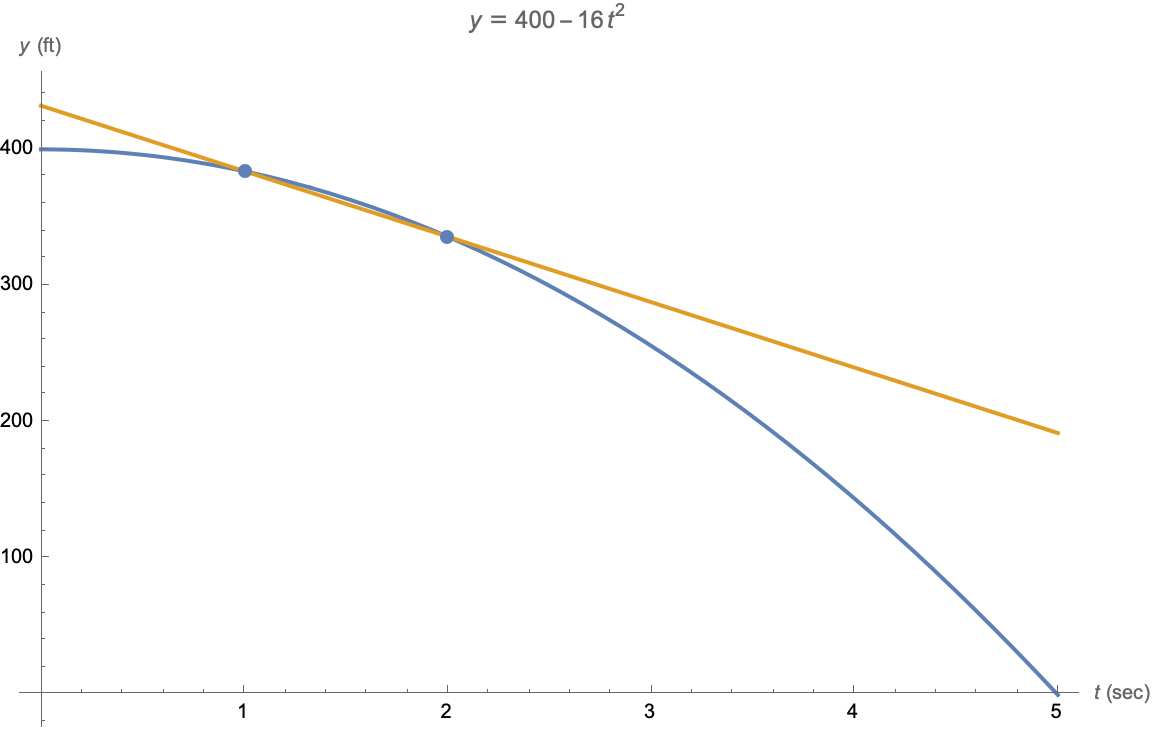
\includegraphics[width=3in]{img/avg_roc1}
\end{flushleft}
\vfill 
\item Compute the average velocity of the stone over the time-interval $[2,3]$. Be sure to give appropriate units.
Then compute an equation for the secant line passing through the graph at $(2,f(2))$ and $(3,f(3))$.
\begin{flushleft}
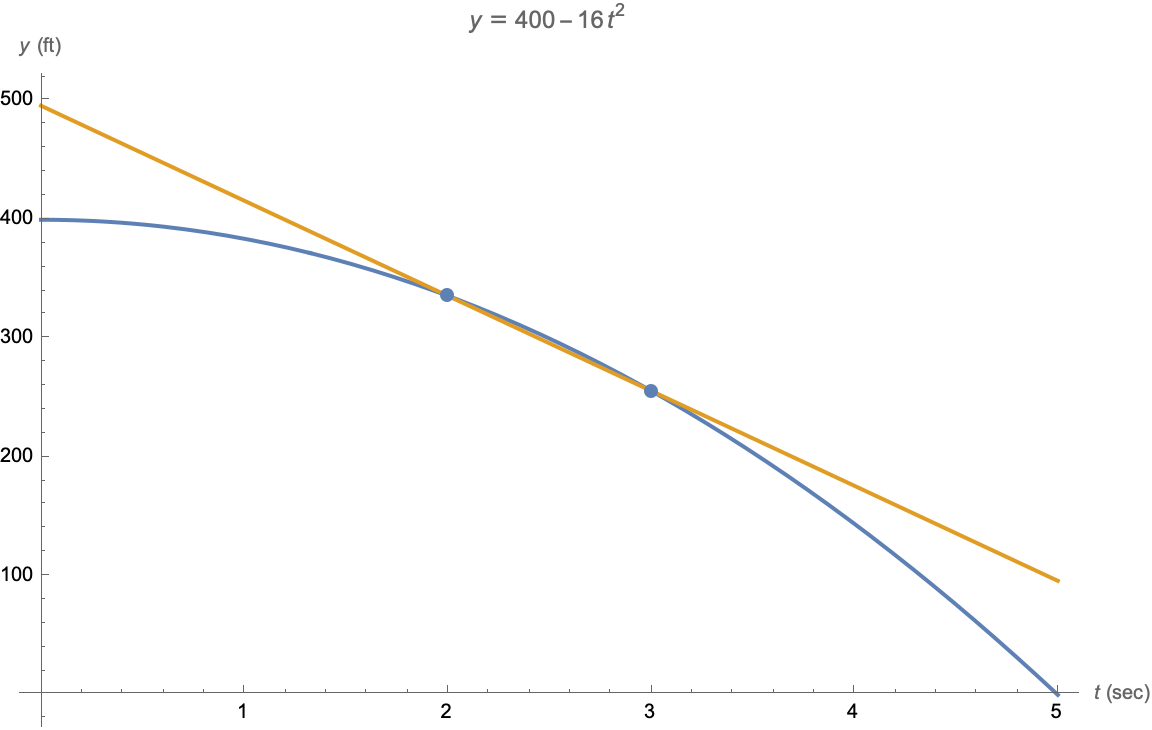
\includegraphics[width=3in]{img/avg_roc2}
\end{flushleft}
\vfill

\newpage

\item What is the average velocity of the stone over the time-interval $[2,2+\Delta t]$ assuming that $\Delta t>0$?
\vfill
\item Use a calculator or Mathematica to fill out the table below.
\begin{table}[H]
\begin{tabular}{|c|c|c|}
\hline
$\Delta t$ \si{(sec)} & $[2,2+\Delta t]$ & $\Delta y/\Delta t$ \si{(ft/sec)}\\
\hline\hline
&&\\
1  & $[2,3]$ &\\
&&\\
\hline
&&\\
0.1 & $[2,2.1]$ & \\
&&\\
\hline
&&\\
0.01 & $[2,2.01]$ & \\
&&\\
\hline
&&\\
0.001 & $[2,2.001]$ & \\
&&\\
\hline
&&\\
0.0001 &$[2,2.0001]$& \\
&&\\
\hline
&&\\
0.00001 &$[2,2.00001]$& \\
&&\\
\hline
&&\\
0.000001 &$[2,2.000001]$& \\
&&\\
\hline
\end{tabular}
\end{table}
\vfill
\newpage
\item What is the average velocity of the stone over the time-interval $[2+\Delta t,2]$ assuming that $\Delta t<0$?
\vfill
\item Use a calculator or Mathematica to fill out the table below.
\begin{table}[H]
\begin{tabular}{|c|c|c|}
\hline
$\Delta t$ \si{(sec)} & $[2+\Delta t,2]$ & $\Delta y/\Delta t$ \si{(ft/sec)}\\
\hline\hline
&&\\
-1  &$[1,2]$ &\\
&&\\
\hline
&&\\
-0.1 &$[2.9,2]$& \\
&&\\
\hline
&&\\
-0.01 &$[2.99,2]$& \\
&&\\
\hline
&&\\
-0.001 &$[2.999,2]$& \\
&&\\
\hline
&&\\
-0.0001 &$[2.9999,2]$& \\
&&\\
\hline
&&\\
-0.00001 &$[2.99999,2]$& \\
&&\\
\hline
&&\\
-0.000001 &$[2.999999,2]$& \\
&&\\
\hline
\end{tabular}
\end{table}
\vfill
\item What do you guess is the velocity of the stone at the instant $t=2$ seconds after it began its fall?
\vfill
\end{enumerate}


\newpage

\begin{mdframed}
\textbf{The big idea of calculus:} Many hard/impossible questions can be answered if we can construct a infinite system of \underline{ever-improving} approximate answers.
The limit is the tool that allows us to ``sneak up" on the exact answer.
\end{mdframed}
\vspace{12pt}
\begin{mdframed}
\textbf{The big idea of limit}:
We say that $f(x)$ approaches the \textbf{limit} $L$ as $x$ approaches $c$, and we write
\begin{equation*}
\lim_{x\to c}f(x) = L,
\end{equation*}
provided that $y$ can be made ``arbitrarily close" to $L$ by taking $x$ ``sufficiently close" (but not equal) to $c$.
\end{mdframed}

\begin{remark}\,
\begin{itemize}
\item This isn't a real definition because of the subjective terms in quotes, but we'll fix that later.
\item The real power of the limit is that it ``does not care" about the value of $y=f(x)$ at $x=c$.
It only cares about what is happening ``on the approach" to $c$.
\item Because of the ``(but not equal) to $c$'' part above, we don't even need $f(x)$ to be defined at $x=c$.
\end{itemize}
\end{remark}
\vfill

\begin{definition}
The \textbf{instantaneous rate of change} of $y=f(x)$ with respect to $x$ at $x=c$ is
\begin{equation*}
\frac{\dee y}{\dee x}\Big|_{x=c} = \lim_{h\to 0}\frac{f(c+h)-f(c)}{h}.
\end{equation*}
Assuming that such a number exists, this is also the slope of the \textbf{tangent} line passing through the curve at $\big(c,f(c)\big)$.
\end{definition}

\begin{example}
Compute the velocity of the falling rock at exactly $t=2$ seconds after the moment it began to fall.
\end{example}

\vfill
\vfill

\newpage


\begin{figure}[H]
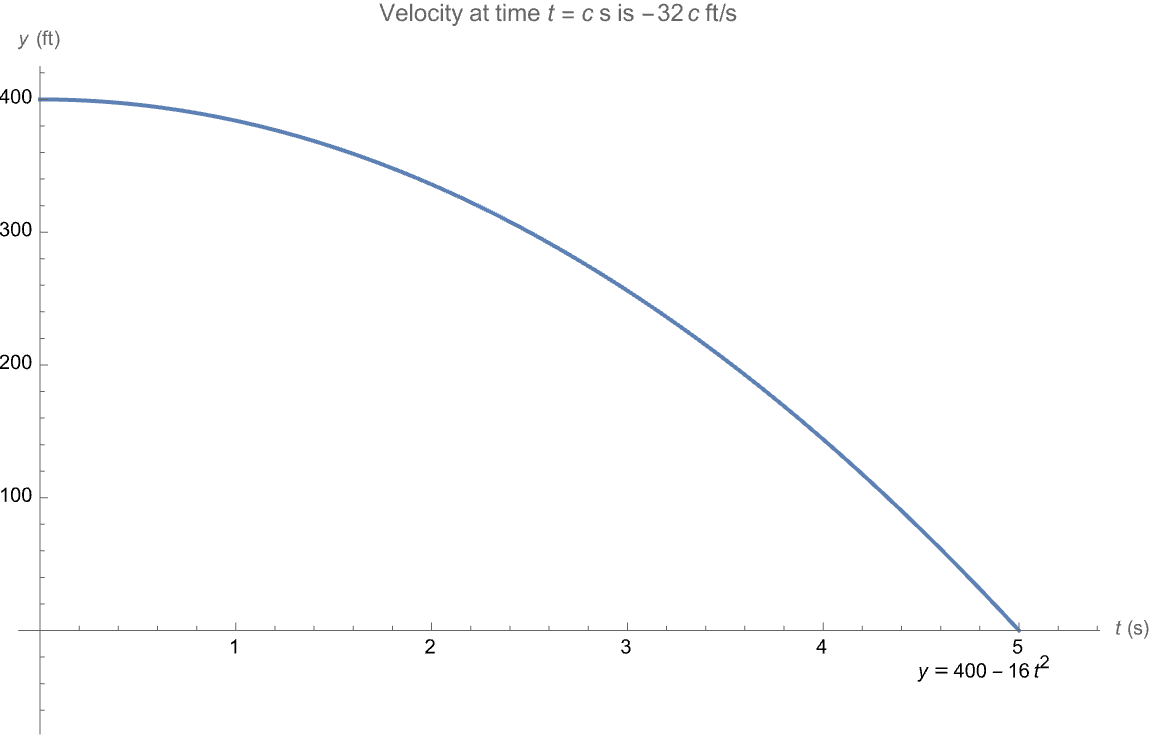
\includegraphics[width=6.5in]{img/roc}
\end{figure}

